\section{Saddle-Point Approaches}\label{sec:lgc.sp}

\subsection{Linear \texorpdfstring{\Track}{}}

It is seemingly unlikely that \LTCCG could be asymptotically optimal according to Fig.~\ref{fig:convergence} despite its decent practical performance. On the other hand, the linear version of \Track seems to be a more plausible candidate of being asymptotically optimal provided that a numerical solver for computing the optimal weights exists. Degenne et al. (2020) provide a Frank-Wolfe-typed heuristic (see Appendix~\ref{app:lgc.approx} for details). No convergence guarantee is given though.

\Track remains unchanged in the linear case, since it only cares about tracking the optimal weights. We hereby recall that the \CT rule consists of playing
\[
    \hat\bx \in \argmax_{i\in[K]} \sum_{t=0}^n \omega_i^{\epsilon_t}(\hat\bmu_t)-T_{t,i}\,,
\]
where $\bomega^\epsilon$ is a $L^\infty$ projection of $\bomega^\star$ onto the simplex $\Sigma_K^\epsilon \eqdef \{\bomega\in [\epsilon,1]^K : \sum_{i=1}^K \omega_i = 1\}$. The draw back of \Track is that we need to compute a plug-in estimate of the optimal weights at each stage, with the current solver it is extremely time-consuming.

\subsection{Saddle-point Frank-Wolfe}
It is natural to look into a saddle-point version of \LGapE (resp. \LTCC) that we call \SLGapE (resp. \SLTCC), as shown in Algorithm~\ref{alg:slgape} (resp. Algorithm~\ref{alg:slt3c}) based on the Frank-Wolfe solver (see Algorithm~\ref{alg:solver} in Appendix~\ref{app:lgc.approx}). We define a so called \emph{active transductive set} as
\begin{align}\label{def:active_transductive}
    \hat\cY(\bx,\btheta) \eqdef \left\{ \frac{(\bx- \bx')}{\left|(\bx-\bx')\transpose\btheta\right|}: \bx'\in\cX/\big\{\bx\big\}  \right\}\,.
\end{align}

\begin{algorithm}[ht]
\centering
\caption{\SLGapE}
\label{alg:slgape}
%\footnotesize
\begin{algorithmic}[1]
    \State {\bfseries Input:} $\delta$
    \State {\bfseries Initialize:} $\mathbf{\tLambda} \leftarrow{} I_d, \mathbf{\Lambda}\leftarrow{} I_d$

   \For{$n \leftarrow 1,2,\cdots$}
        \State $\mathbf{\hat{\bx}}\in\argmax_{\bx\in\cX}  \norm{\bx}_{\mathbf{\Lambda}^{-1} \mathbf{\tLambda} \mathbf{\Lambda}^{-1} }^2$
        \State $\hat{\bx}^{(1)} \leftarrow \argmax_{\bx\in\cX} \bx\transpose\hat\btheta^{\lambda}_n$
        \State $\hat{\bx}^{(2)} \leftarrow \argmax_{\bx\neq\hat{\bx}^{(1)}} (\bx-\hat{\bx}^{(1)})\transpose\hat\btheta^{\lambda}_n + \sqrt{2\beta(n,\delta)}\normm{\hat{\bx}^{(1)}-\bx}_{\bLambda^{-1}}$
        \State $B_n \leftarrow \max_{\bx\neq\hat{\bx}^{(1)}} (\bx-\hat{\bx}^{(1)})\transpose\hat\btheta^{\lambda}_n + \sqrt{2\beta(n,\delta)}\normm{\hat{\bx}^{(1)}-\bx}_{\bLambda^{-1}}$
        \If{$B_n \leq 0$}
            \State \Return $\hat{\bx}^{(1)}$
        \EndIf
        \State $\hat\by \leftarrow{} \dfrac{(\hat{\bx}^{(1)}- \hat{\bx}^{(2)})}{(\hat{\bx}^{(1)}-\hat{\bx}^{(2)})\transpose\btheta}$
        \State $\bLambda\leftarrow{} \mathbf{\Lambda}+ \mathbf{\hat\bx}\mathbf{\hat\bx}\transpose$
		\State $\mathbf{\tLambda} \leftarrow{} \mathbf{\tLambda} + \mathbf{\hat\by}\mathbf{\hat\by}\transpose$
		\State \texttt{evaluate arm} $\hat{\bx}$
	    \State \texttt{update mean and variance according to \eqref{eq:update_mean} and \eqref{eq:update_variance}}
	    \State $n = n+1$
   \EndFor
\end{algorithmic}
\end{algorithm}

\begin{algorithm}[ht]
\centering
\caption{Sampling rule (\SLTCC)}
\label{alg:slt3c}
%\footnotesize
\begin{algorithmic}[1]
   \State {\bfseries Initialize:} $\mathbf{\tLambda} \leftarrow{} I_d, \mathbf{\Lambda}\leftarrow{} I_d$

   \For{$n \leftarrow 1,2,\cdots$}
        \State \texttt{sample} $\btheta \sim \Pi_n$
        \State $\mathbf{\hat{\bx}}\in\argmax_{\bx\in\cX}  \norm{\bx}_{\mathbf{\Lambda}^{-1} \mathbf{\tLambda} \mathbf{\Lambda}^{-1} }^2$
        \State $\mathbf{\hat{\by}}\in\argmax_{\by\in\hat\cY(\hat\bx,\btheta)}\normm{\by}^2_{\mathbf{\Lambda}^{-1}}$
        \State $\mathbf{\Lambda}\leftarrow{} \mathbf{\Lambda}+ \mathbf{\hat\bx}\mathbf{\hat\bx}\transpose$
		\State $\mathbf{\tLambda} \leftarrow{} \mathbf{\tLambda} + \mathbf{\hat\by}\mathbf{\hat\by}\transpose$
		\State \texttt{evaluate arm} $\hat{\bx}$
	    \State \texttt{update mean and variance according to \eqref{eq:update_mean} and \eqref{eq:update_variance}}
	    \State $n = n+1$
   \EndFor
\end{algorithmic}
\end{algorithm}

\subsection{Experiment illustrations}

\paragraph{Experiments for classical bandits} 
\LTCCG can be particularized to the classic BAI setting (that corresponds to choosing the canonical basis as contexts). In that case, the selection rule in Line 6 of Algorithm~\ref{alg:lt3cg} corresponds to choosing the least pulled arm between the two candidates. 

We investigate whether \LTCCG could be optimal in the classical bandit setting with some preliminary experiments. In particular, we call the derived algorithm \TCCG. See Fig.~\ref{fig:convergence} for a comparison against the asymptotically optimal \DT rule and the oracle. 


\begin{figure}[ht]
    \centering
    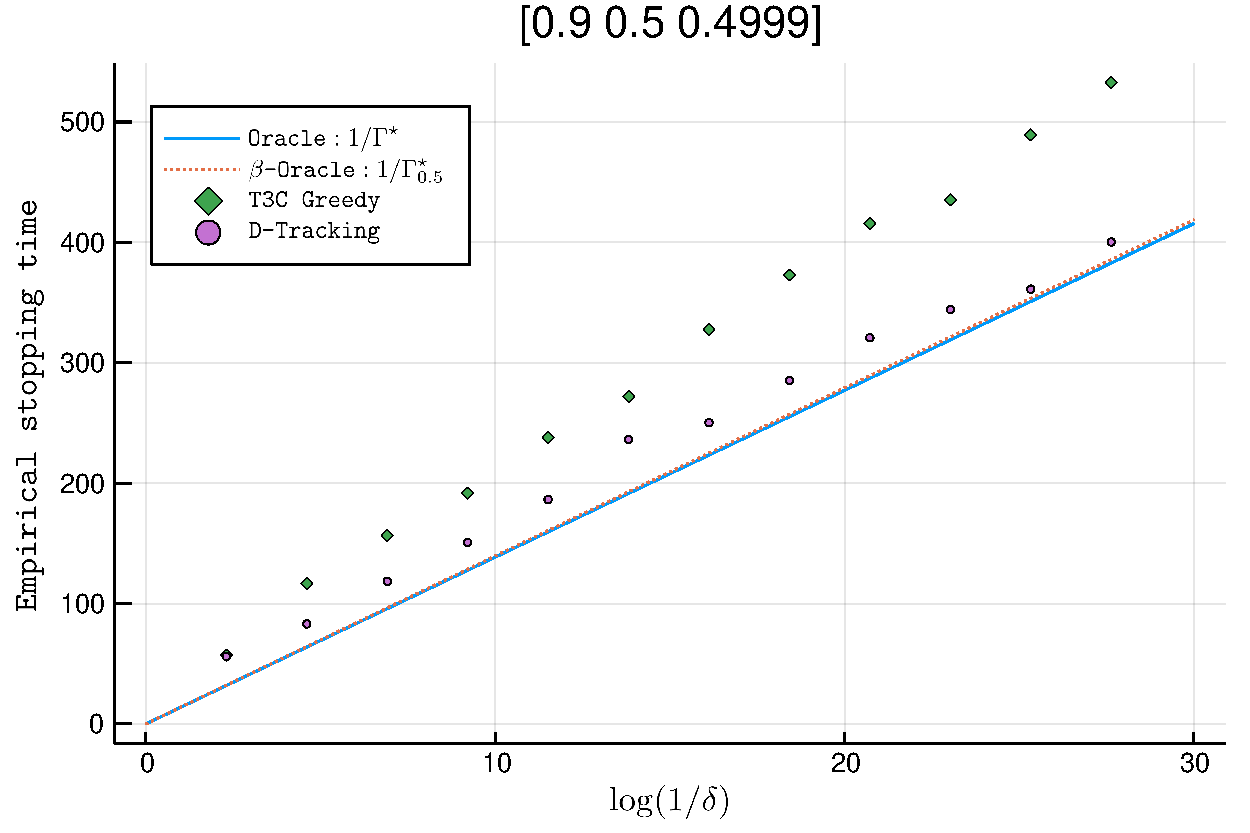
\includegraphics[width=0.49\textwidth]{Chapter4/img/res1.pdf}
    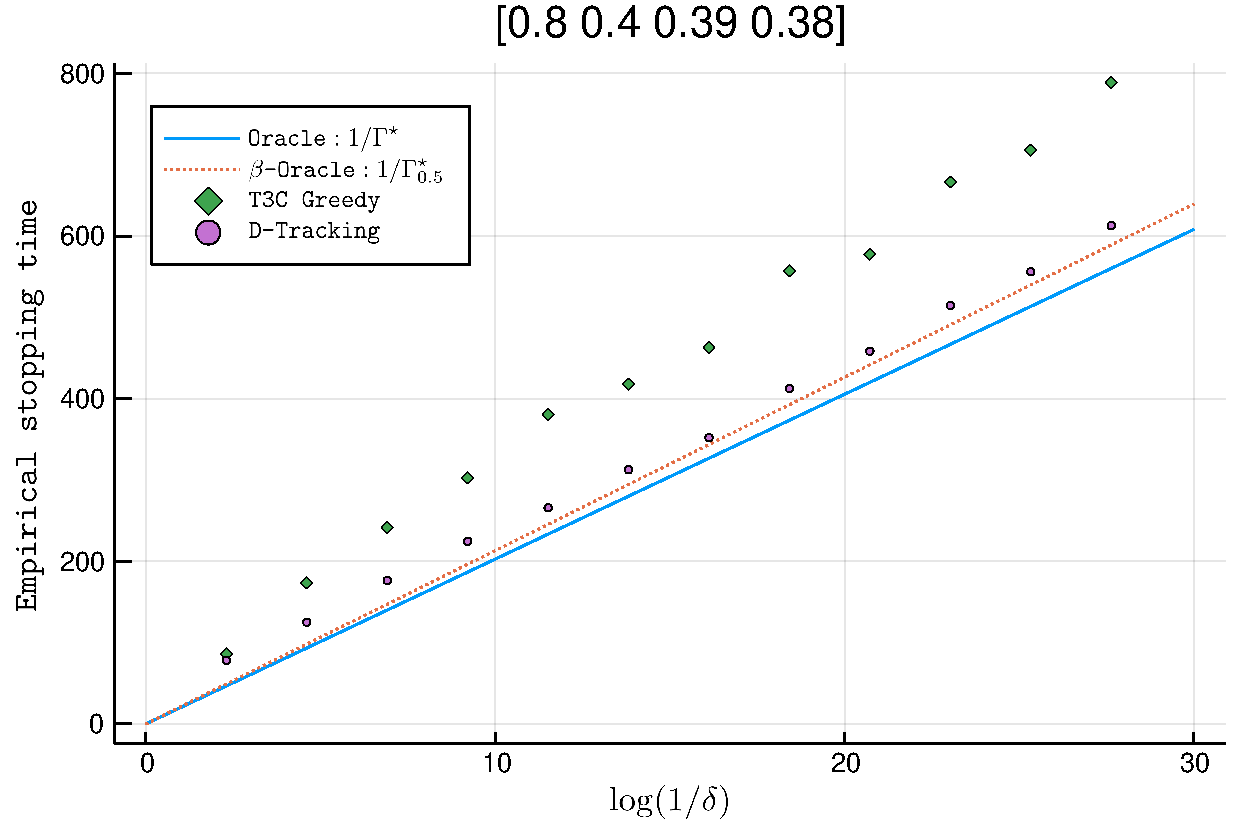
\includegraphics[width=0.49\textwidth]{Chapter4/img/res2.pdf}
    \caption{\TCCG{} versus \Track{} for different value of $\delta$.}
    \label{fig:convergence}
\end{figure}

\paragraph{\LTCCG}
We compare its performance to \LGapE over the aforementioned pathological instance with $d=2$, $\lambda=2$ and two values of $\alpha$. More precisely, we report in Table~\ref{table:pulls1} the total number of pulls and also the number of pulls allocated to each arm for each of the sampling rules. The results confirm our intuition in the previous section. 

\begin{table*}[ht]
\centering
\begin{tabular}{|c|c|c|}
 \hline
 & \LTCCG & \LGapE \\
 \hline
 \textbf{$\bx_1=(1,0)\transpose$} & $1783.1$ & $5844.4$ \\
 \hline
 \textbf{$\bx_2=(0,1)\transpose$} & $357009.0$ & $1169260.5$ \\
 \hline
 \textbf{$\bx_3=(\cos(0.01),\sin(0.01)\transpose)$} & $1.0$ & $1.0$ \\
 \hline
 \textbf{Total} & $\textbf{358793.1}$ & $1175105.9$ \\
 \hline
\end{tabular}
\caption{Average number of pulls of each arm ($d=2, \delta=0.1$).}
\label{table:pulls1}
\end{table*}

\begin{table*}[ht]
\centering
\begin{tabular}{|c|c|c|c|}
 \hline
 & \LTCC ($\beta=1/2$) & \LTCCG & \LGapE \\
 \hline
 \textbf{$\bx_1=(1,0)\transpose$} & $131.3$ & $24.9$ & $26.3$ \\
 \hline
 \textbf{$\bx_2=(0,1)\transpose$} & $3.3$ & $60.8$ & $63.4$ \\
 \hline
 \textbf{$\bx_3=(\cos(\pi/4),\sin(\pi/4)\transpose)$} & $133.4$ & $1.0$ & $1.0$ \\
 \hline
 \textbf{Total} & $268.0$ & $\textbf{86.7}$ & $89.7$ \\
 \hline
\end{tabular}
\caption{Average number of pulls of each arm ($d=2, \delta=0.1$).}
\label{table:pulls2}
\end{table*}

We also compare the impact of the dimension $d$ over the performance of our sampling rule and $\LGapE$. We run experiments on the same instance with a value of the angle set to $\alpha=0.1$. This time we let the dimension $d$ varying from 2 to 6. \LTCC{} is always better and the performance gap increases with the dimension. Thus, our algorithm seems to be more robust to the dimension.

\begin{figure}[ht]
    \centering
    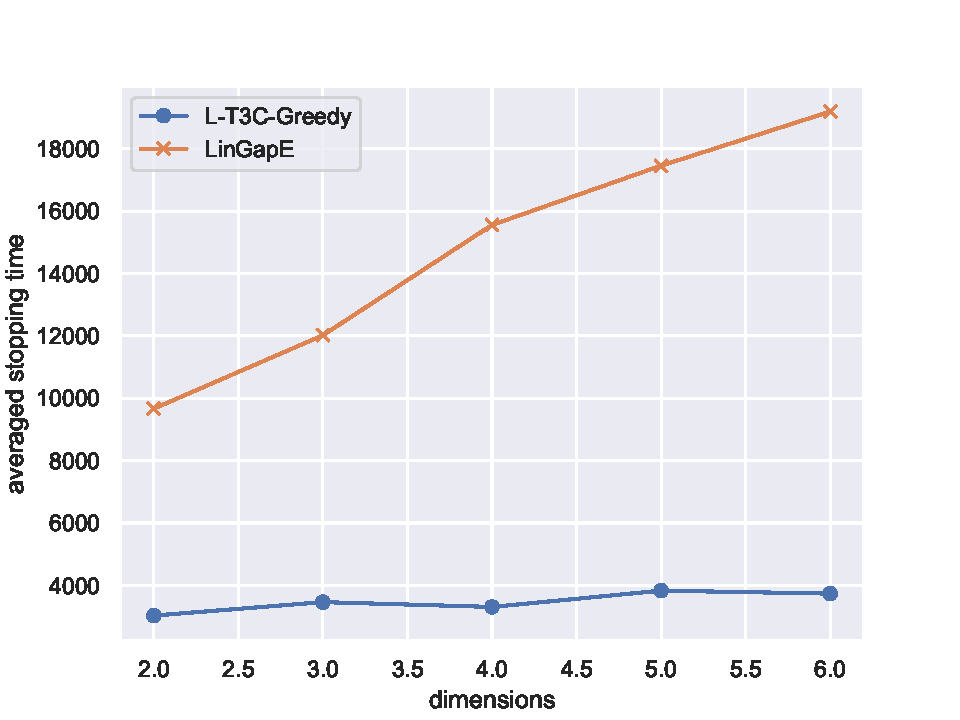
\includegraphics[width=0.45\textwidth]{Chapter4/img/dims.pdf}
    \caption{Comparison of the sample complexity of \LTCCG{} and \LGapE{} on the pathological instance in $\R^d$ for different values of $d$.}
    \label{fig:dims}
\end{figure}

\paragraph{Saddle-point sampling rules}
We now compare our saddle-point-based algorithms against \LGapE. To make a fair comparison, we use always the same exploration rate for all the stopping rules. Indeed the stopping rules are equivalent if they keep the same exploration rate as argued by Degenne et al. (2020). We first use the previous pathological instance with $\lambda=1$, the results are reported as box plots of average stopping time in Fig.~\ref{fig:exp1}.

\begin{figure}[ht]
    \centering
    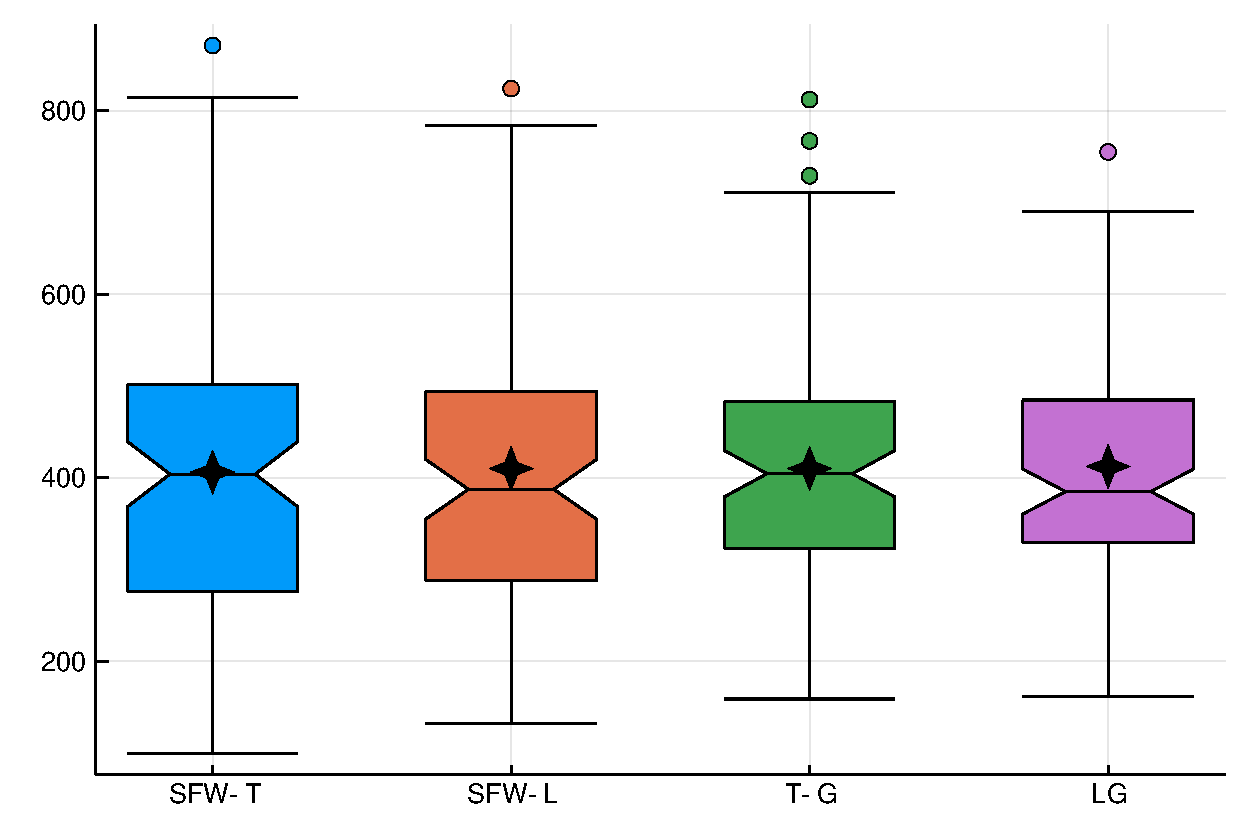
\includegraphics[width=0.49\textwidth]{Chapter4/img/exp_sin_-0000001}
    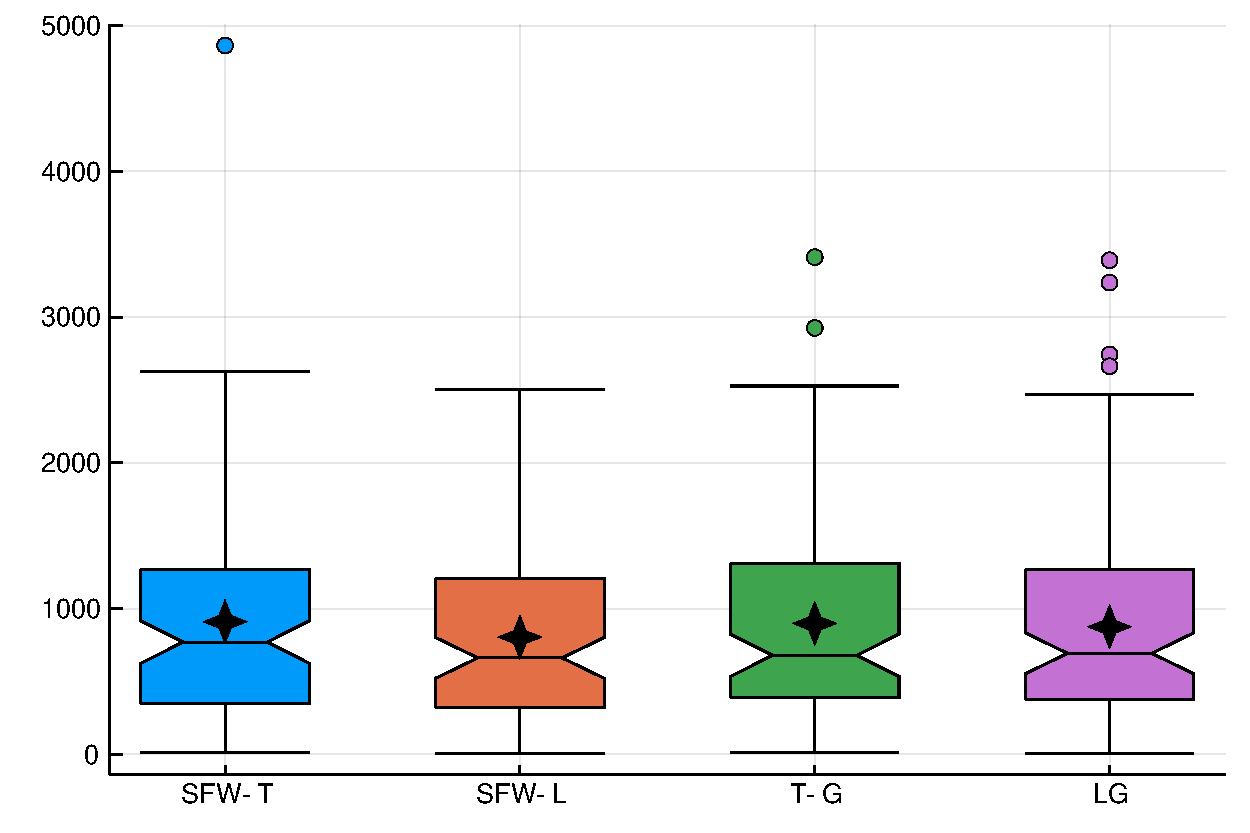
\includegraphics[width=0.49\textwidth]{Chapter4/img/exp_sin_-1}
    \caption{Average stopping time (Left: $d=2,\alpha=\pi/4,\delta=0.0000001$, Right: $d=2,\alpha=0.1,\delta=0.1$), with SFW-T = \SLTCC, SFW-L = \SLGapE, T-G = \LTCC, LG = \LGapE.}
    \label{fig:exp1}
\end{figure}

\subsection{Additional experiments}

In this section, we always keep each context normalized. We provide more experimental illustrations on different types of problems.

\paragraph{Arms with mild gaps}
We construct a set of $n$ arms proposed by~\cite{fiez2019transductive}: $\bx_1=(1,0)\transpose$, $\bx_2=(\cos(3\pi/4),\sin(3\pi/4))\transpose$, and for $i = 3,\ldots,n$, $\bx_i=(\sin(\pi/4+\phi_i),\cos(\pi/4+\phi_i))\transpose$ where $\phi_i\sim\cN(0,0.09)$. We fix the true regression parameter $\theta^\star$ to be $\be_1$. This set of arms has some nice properties, that $\bx_1$ is the optimal arm, and $\bx_2$ is the arm that gives more information on identifying the best arm. We first report results with a moderate $n=6$ as an example where the generated expected means are $[1.0, -0.71, 0.84, -0.95, 0.93, 0.99]$.

\begin{table*}[t!]
\centering
\def\arraystretch{1.2}
\begin{tabular}{|c|c|c|c|}
 \hline
 & \LTCC & \LTCCG & \LGapE \\
 \hline
 \textbf{$\bx_1=(1,0)\transpose$} & $170872.19$ & $1.06$ & $1.13$ \\
 \hline
 \textbf{$\bx_2=(\cos(3\pi/4),\sin(3\pi/4))\transpose$} & $1.25$ & $1.0$ & $1.0$ \\
 \hline
 \textbf{$\bx_3=(\sin(\pi/4+\phi_3),\cos(\pi/4+\phi_3))\transpose$} & $92.18$ & $28693.26$ & $120657.6$ \\
 \hline
 \textbf{$\bx_4=(\sin(\pi/4+\phi_4),\cos(\pi/4+\phi_4))\transpose$} & $1.12$ & $26197.03$ & $110157.63$ \\
 \hline
 \textbf{$\bx_5=(\sin(\pi/4+\phi_5),\cos(\pi/4+\phi_5))\transpose$} & $77.04$ & $1.0$ & $1.0$ \\
 \hline
 \textbf{$\bx_6=(\sin(\pi/4+\phi_6),\cos(\pi/4+\phi_6))\transpose$} & $170892.82$ & $1.36$ & $1.83$ \\
 \hline
 \textbf{Total} & $341936.6$ & $\textbf{54894.71}$ & $230820.19$ \\
 \hline
\end{tabular}
\caption{average number of pulls of each arm ($d=2, \delta=0.1$).}
\label{table:pulls3}
\end{table*}
